\section{Development \& Results}
\begin{frame}{Development \& Results}
Development is divided into:
\begin{itemize}
    \item EEG MI Classifier
    \item Dataset Augmentation Technique
    \item Virtual Environment
    \item Project Testing Pipeline
\end{itemize}
\end{frame}

\begin{frame}{EEG MI Classifier - Baseline Methods}
\begin{itemize}
    \item \textbf{CSP + LDA}: Common Spatial Patterns + Linear Discriminant Analysis
    \item \textbf{TGSP + SVM}: Tangent Space Projection + Support Vector Machine
    \item \textbf{MDM}: Minimum Distance Mean
    \item \textbf{EEGNetV4}: Convolutional Neural Network for Motor Imagery Classification
\end{itemize}
\end{frame}
\begin{frame}{EEG MI Classifier - Baseline Methods - Results}
    \begin{figure}[htpb!]
        \centering
        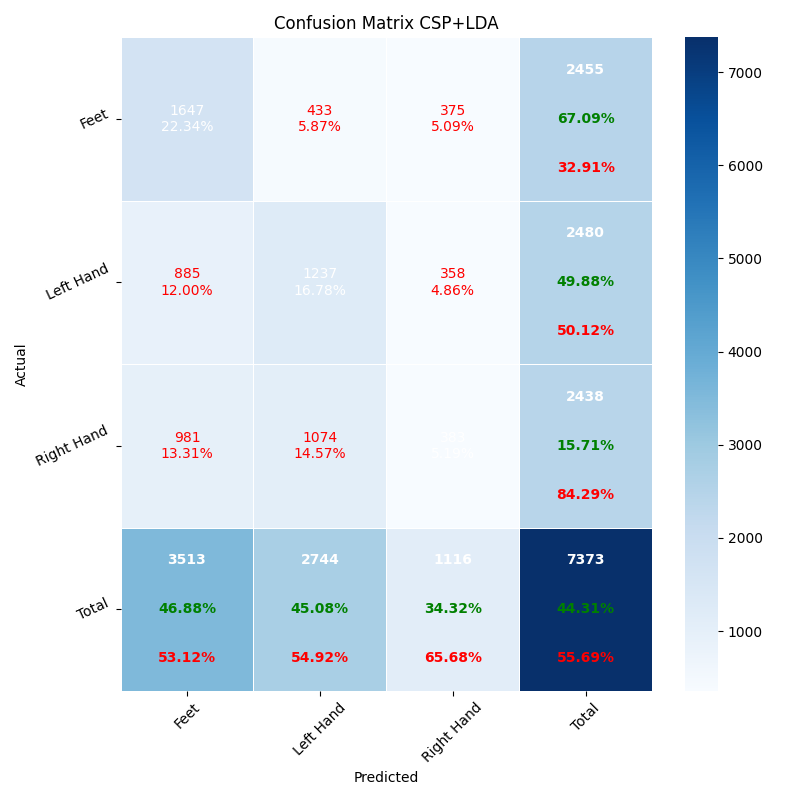
\includegraphics[width=0.30\textwidth]{figures/classification/confusion_matrix_csp_lda}
        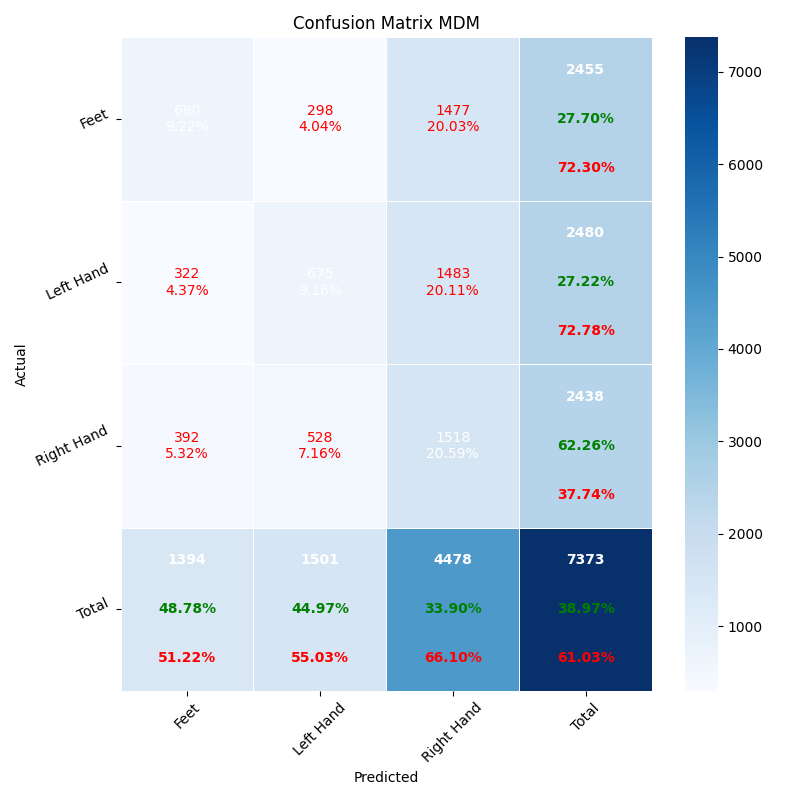
\includegraphics[width=0.30\textwidth]{figures/classification/confusion_matrix_mdm}
        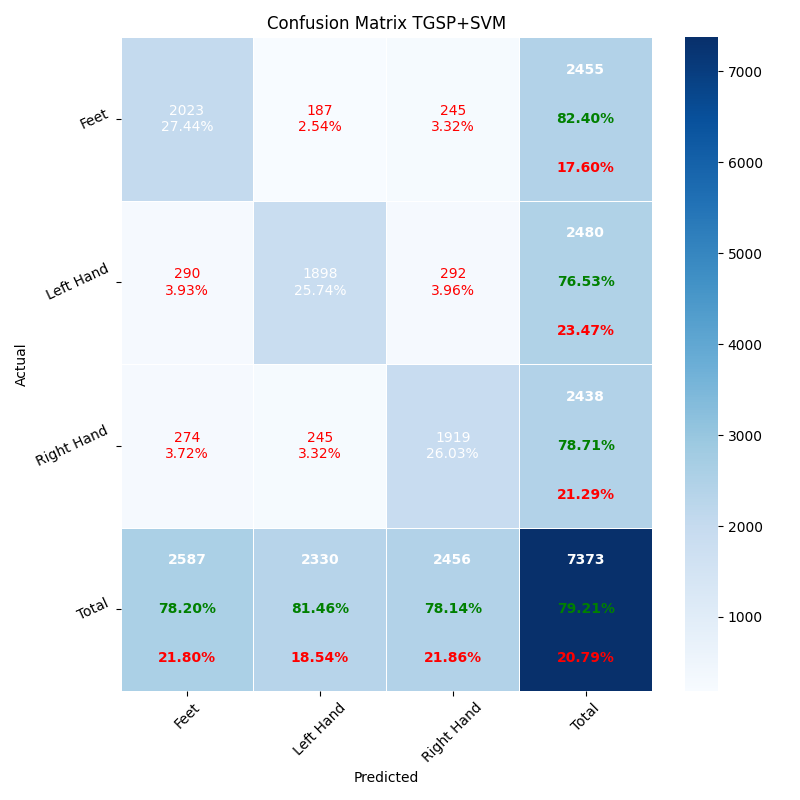
\includegraphics[width=0.30\textwidth]{figures/classification/confusion_matrix_tgsp_svm}
        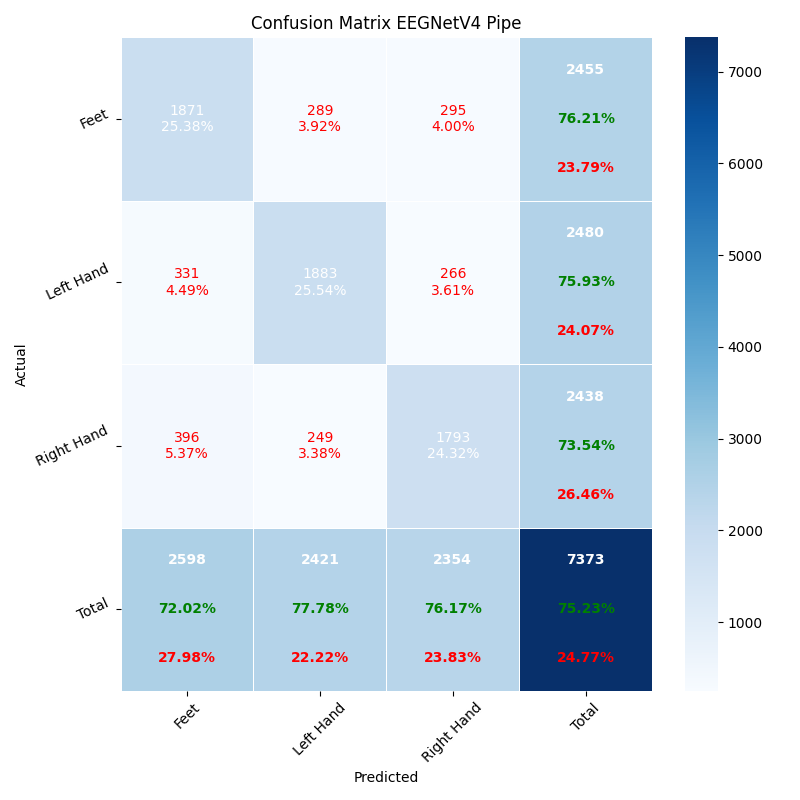
\includegraphics[width=0.30\textwidth]{figures/classification/confusion_matrix_eegnetv4_pipe}
        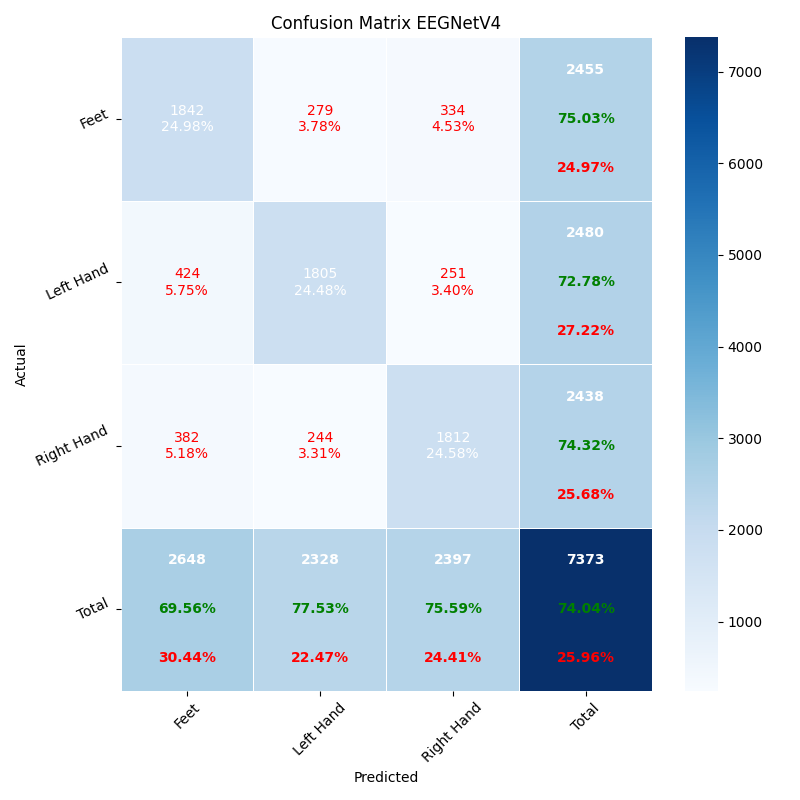
\includegraphics[width=0.30\textwidth]{figures/classification/confusion_matrix_eegnetv4}
    \end{figure}
\end{frame}

\begin{frame}{EEG MI Classifier - Proposed Method}
    From ``\textbf{Deep temporal networks for EEG-based motor imagery recognition.}'' by \textit{Sharma N. et al.} (2023) I used and adapted: 
    \begin{itemize}
        \item LSTM-based Approach
        \item Transformer-based Approach
    \end{itemize}
    % \red{NOTE: Not sure if I should present something new or if I can use something from the literature review.}
\end{frame}
\begin{frame}{EEG MI Classifier - Proposed Method - Results}
    \begin{figure}[htpb!]
        \centering
        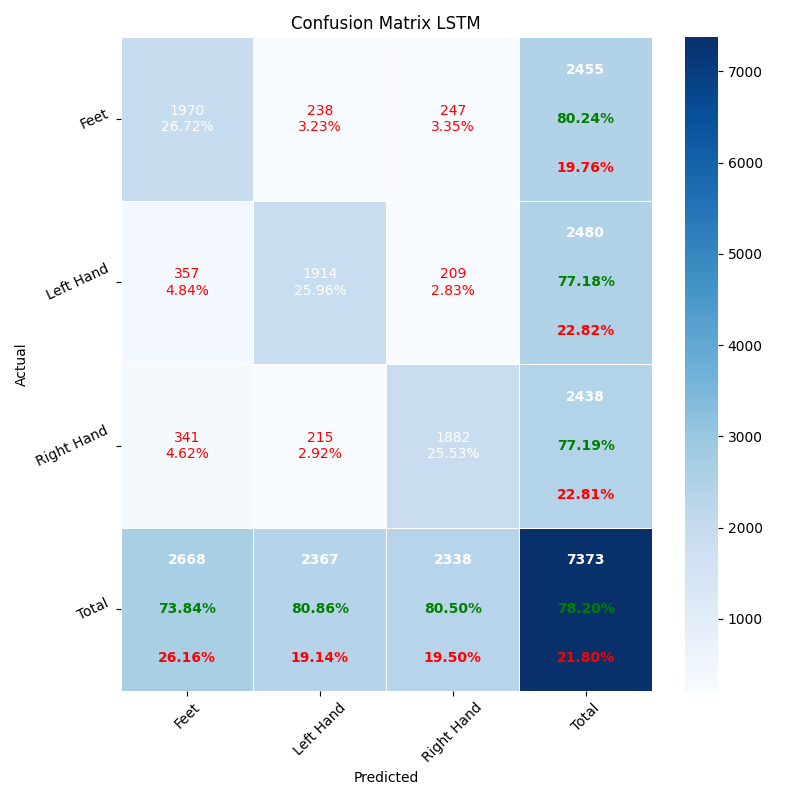
\includegraphics[width=0.49\textwidth]{figures/classification/confusion_matrix_lstm}
        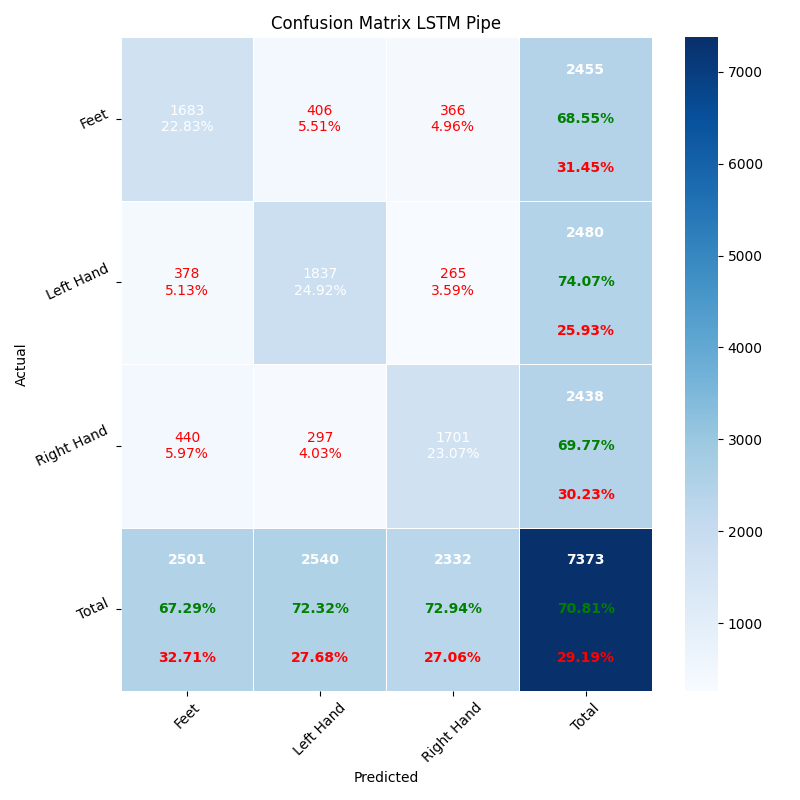
\includegraphics[width=0.49\textwidth]{figures/classification/confusion_matrix_lstm_pipe}
    \end{figure}
\end{frame}

\begin{frame}{Dataset Augmentation - GAN Based}
    From ``\textbf{EEGFuseNet: Hybrid Unsupervised Deep Feature Characterization and Fusion for High-Dimensional EEG With an \#Application to Emotion Recognition.}'' by \textit{Z. Liang et al.} (2021) I used and trained the network:
    \begin{itemize}
        \item GAN based Approach $\rightarrow{}$ EEGFuseNet
    \end{itemize}
\end{frame}
\begin{frame}{Dataset Augmentation - GAN Based - Results}
    \begin{figure}[htpb!]
        \centering
        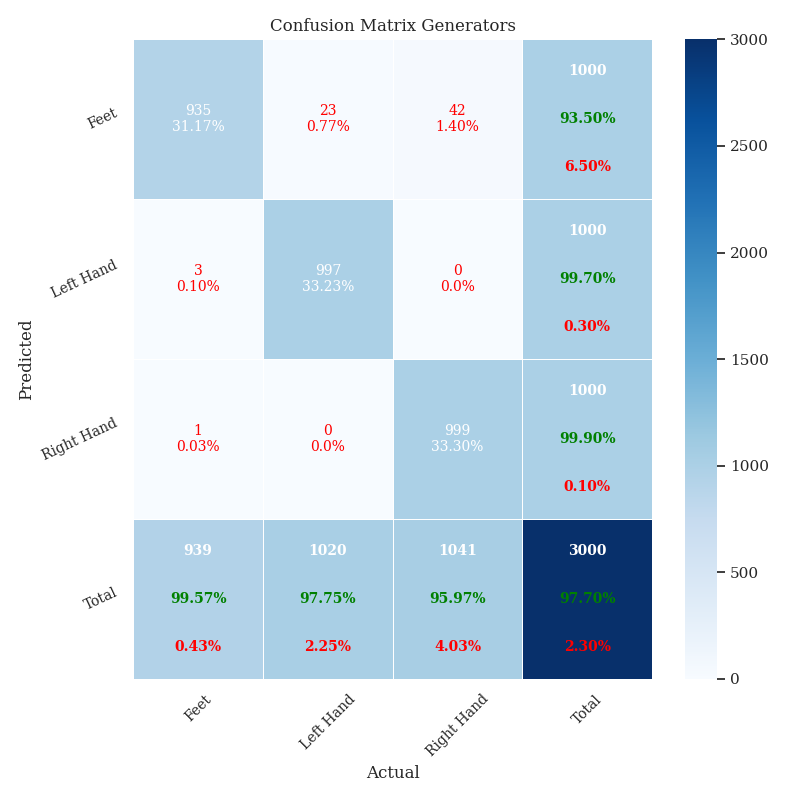
\includegraphics[width=0.55\textwidth]{figures/augmentation/gan/confusion_matrix_generators_generators_using_LSTMNet_0.5943600867678959.pkl.png}
    \end{figure}
\end{frame}

\begin{frame}{Dataset Augmentation - Stochastic Methods}
    From ``'' I created a script to generate data using:
    \begin{itemize}
        \item Stochastic Noise Injection Approach $\rightarrow{}$ Good Results
        \item Stochastic Generation Approach $\rightarrow{}$ Bad Results
    \end{itemize}
\end{frame}
\begin{frame}{Dataset Augmentation - Stochastic Methods - Results}
    \begin{minipage}{0.49\textwidth}
        \begin{figure}[htpb!]
            \centering
            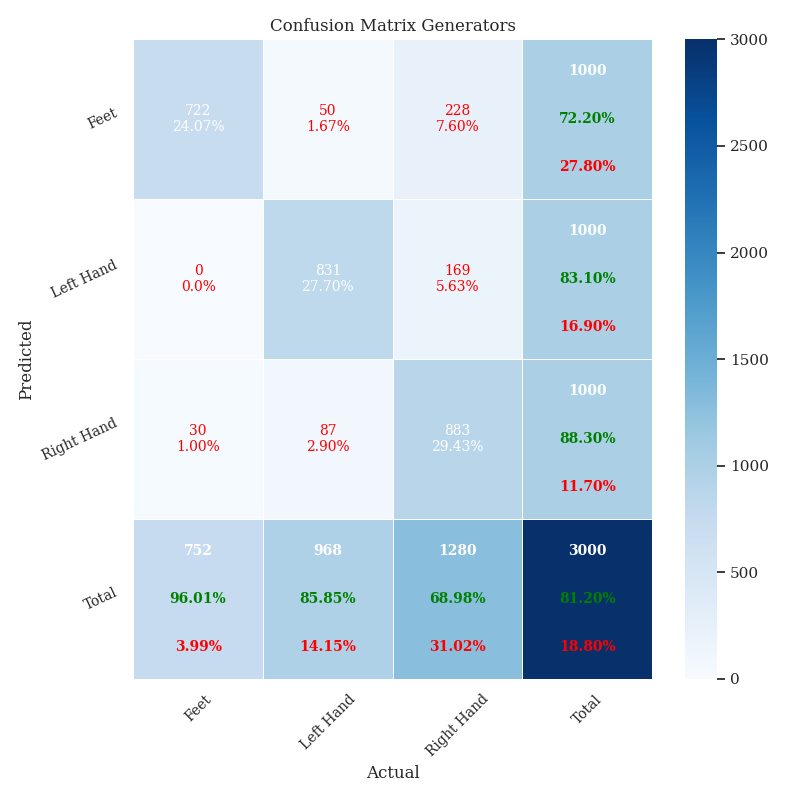
\includegraphics[width=\textwidth]{figures/augmentation/stochastic/confusion_matrix_generators_2024_03_30_18_00_20_noise_injector_using_LSTMNet_0.5943600867678959.pkl.png}
            \caption{Noise Injector}
        \end{figure}
    \end{minipage}
    \begin{minipage}{0.49\textwidth}
        \begin{figure}[htpb!]
            \centering
            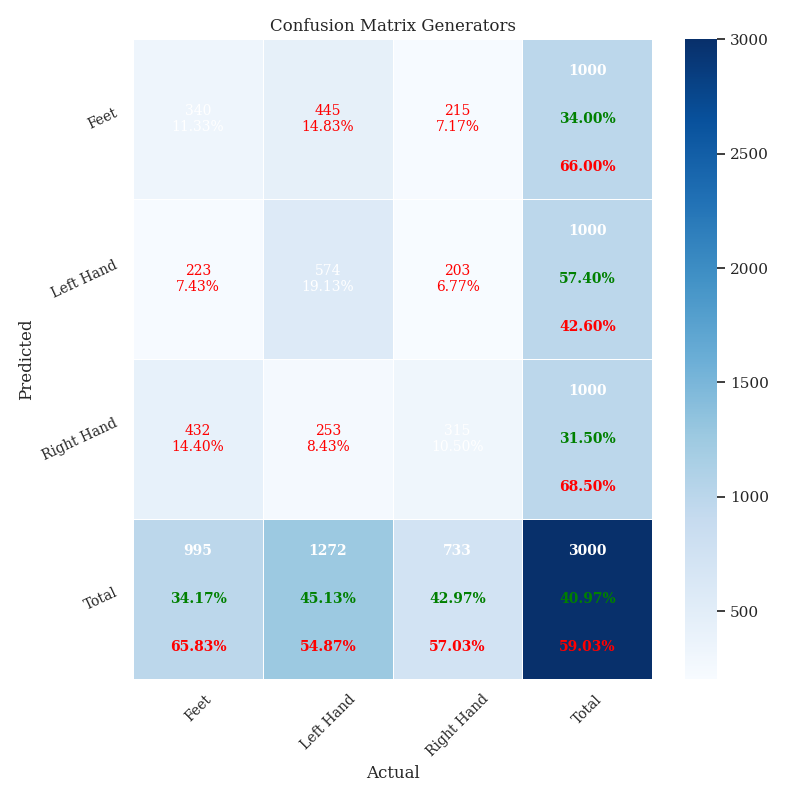
\includegraphics[width=\textwidth]{figures/augmentation/stochastic/confusion_matrix_generators_2024_03_30_18_01_19_random_sampler_using_LSTMNet_0.5943600867678959.pkl.png}
            \caption{Random Sampling}
        \end{figure}
    \end{minipage}
\end{frame}

\begin{frame}{Virtual Environment}
\begin{itemize}
    \item Unity3D based Environment
    \item Infinite Runner (like Temple Run)
\end{itemize}
\end{frame}

\begin{frame}{Project Testing Pipeline}
    \begin{itemize}
        \item Keyboard Controls (W/Space, A, D)
        \item EEG Signals Generation (Feet, Left Hand, Right Hand)
        \item Signal Classification
        \item Classification Transmission (Via WebSocket)
        \item Virtual Character Control
    \end{itemize}
\end{frame}

\begin{frame}{Sample Gameplay}
    \begin{figure}[htpb!]
        \centering
        \href{https://youtu.be/3T2kwwnvs3c}{%
        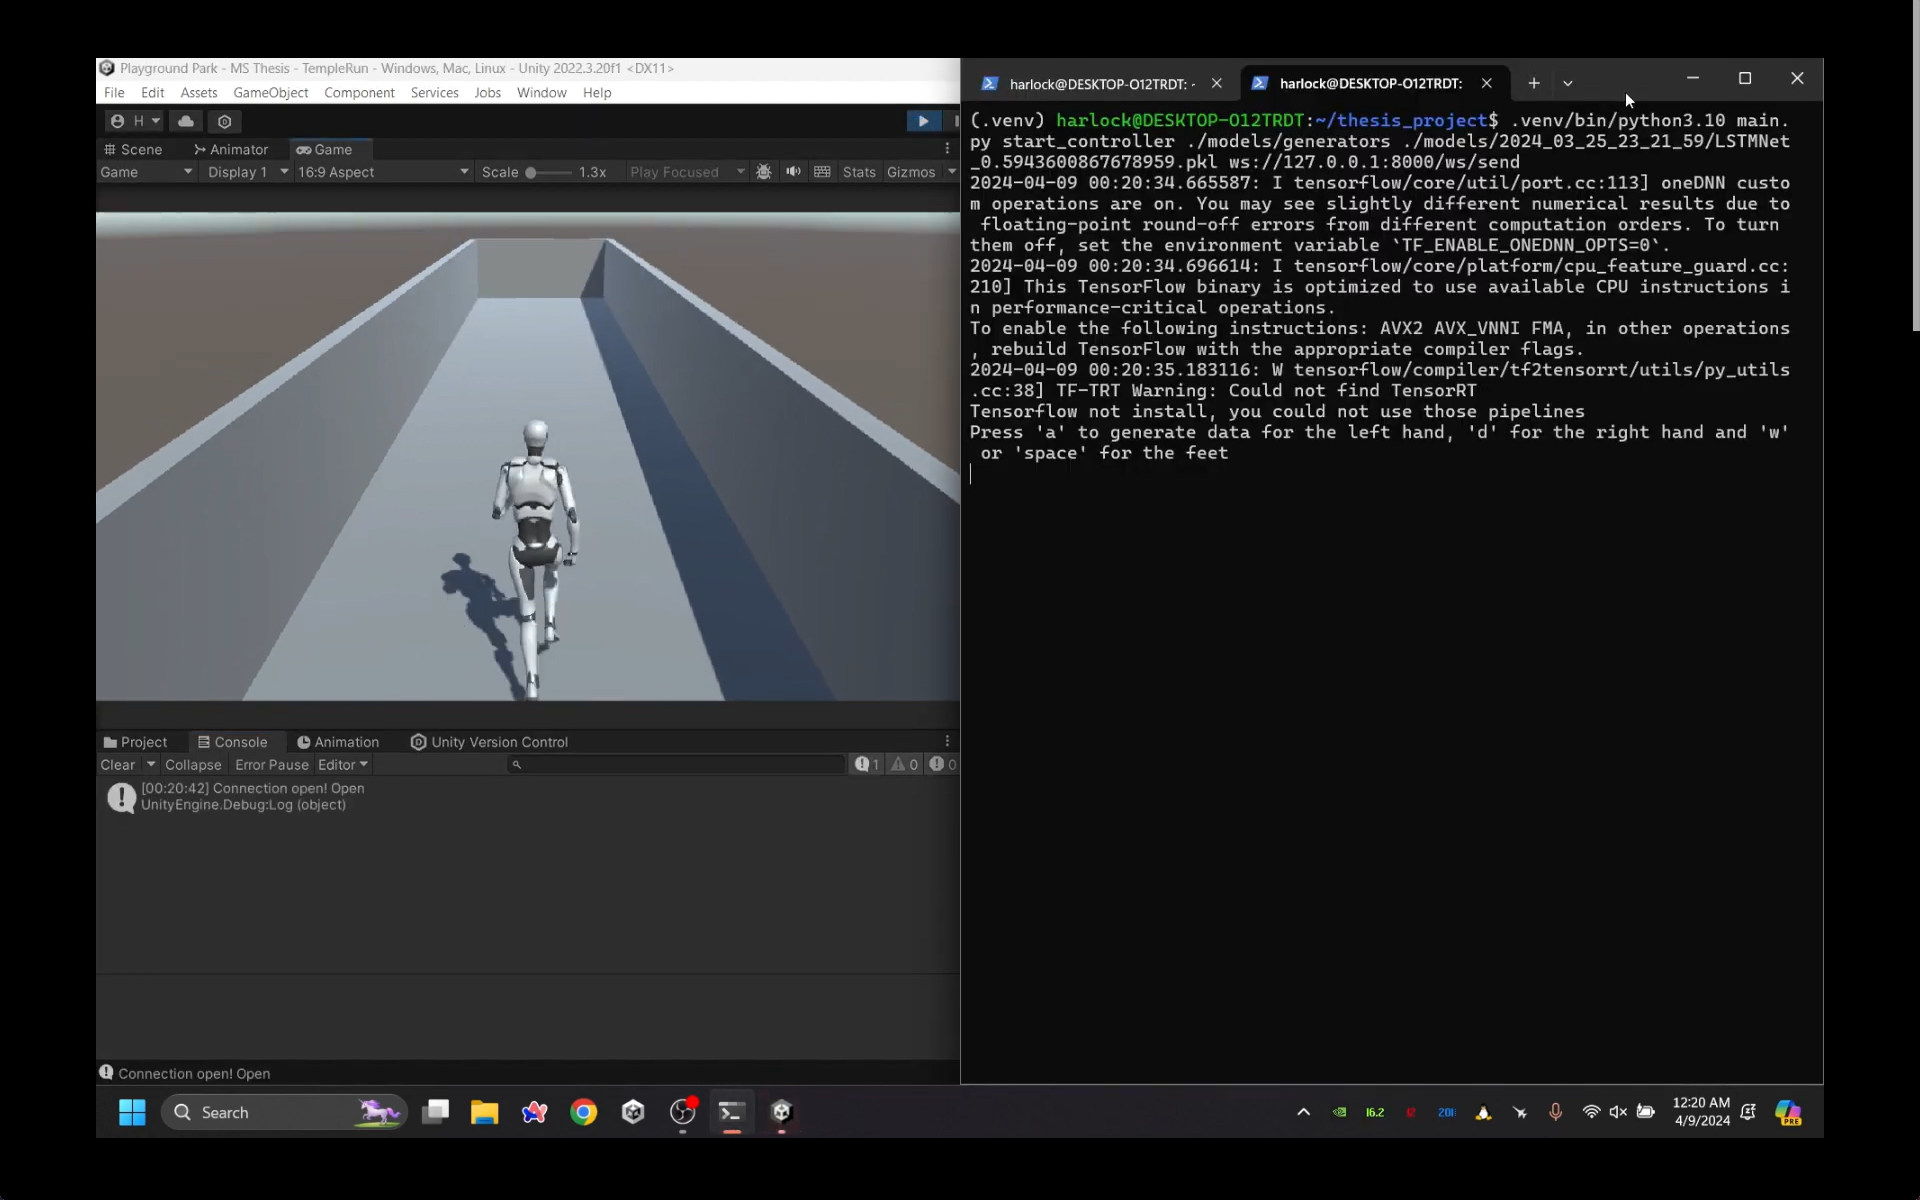
\includegraphics[width=0.8\textwidth]{figures/gameplay/thesisGameplayThumbnail}%
        }
    \end{figure}
\end{frame}